\documentclass{beamer}
\usetheme{Frankfurt}

\usepackage[utf8]{inputenc}
\usepackage[T1]{fontenc}
\usepackage{polski}

\usepackage{amsmath}
\usepackage[]{algorithm2e}
\usepackage{minted}
\usepackage{tikz}

\usetikzlibrary{arrows, shapes}

\title{The intended yet unwanted C++ use cases}
\author{Michał Pletty}

\begin{document}

\frame{\titlepage}

\begin{frame}
    \frametitle{table of contents}
    \tableofcontents
\end{frame}

\section{goal}

\begin{frame}
    \frametitle{usual examples}
    \begin{itemize}
        \item ridiculous
        \item unreal
        \item over engineered
        \item play to their strengths
    \end{itemize}
\end{frame}

\begin{frame}[fragile]
    \frametitle{over engineered}
        \begin{minted}{c++}
const std::vector<T> queue;
    \end{minted}
    \begin{minted}{c++}
for(const auto it = queue.rbegin();
    it != queue.rend(); it++)
{
    cout << to_string(i) << endl;
}
    \end{minted}
    \begin{minted}{c++}
for(const auto & i : reverse(queue))
{
    cout << to_string(i) << endl;
}
    \end{minted}
\end{frame}

\begin{frame}[fragile]
    \frametitle{helper structures}
    \begin{minted}{c++}
template<typename T>
struct reverse_wrapper
{
    T & iterable;
};

template<typename T>
reverse_wrapper<T> reverse(T & t)
{
    return {t};
}
    \end{minted}
\end{frame}

\begin{frame}[fragile]
    \frametitle{helper functions}
    \begin{minted}{c++}
template<typename T>
auto begin(reverse_wrapper<T> & wrapper)
{
    return std::rbegin(wrapper.iterable);
}

template<typename T>
auto end(reverse_wrapper<T> & wrapper)
{
    return std::rend(wrapper.iterable);
}
    \end{minted}
\end{frame}

\begin{frame}[fragile]
    \frametitle{play to their strengths}
        \begin{minted}{c++}
const std::vector<float> data;
    \end{minted}
    \begin{minted}{c++}
float sum = 0;
for(float x : data)
{
    sum += x;
}
    \end{minted}
    \begin{minted}{c++}
float sum = std::accumulate(
    std::begin(data),
    std::end(data),
    0.0
);
    \end{minted}
    \begin{itemize}
        \item <2-> what is $0.0$ ?
        \item <3-> why use magic number ?
    \end{itemize}
\end{frame}

\begin{frame}
    \frametitle{extensibility}
    \begin{itemize}
        \item<+-> no! I want the job done now!
        \item<+-> correctness over extensions
        \item<+-> polimorfizm is no longer cool
        \item<+-> polimorfizm != dynamic dispatch
        \item<+-> composition over inheritance
    \end{itemize}
\end{frame}

\begin{frame}
    \frametitle{plan}
    \begin{enumerate}
        \item meaningful and nontrivial application
        \item solve problem in C
        \item solve problem in C++
        \item mutate to improve
        \begin{enumerate}
            \item correctness
            \item readability
            \item maintainability
        \end{enumerate}
    \end{enumerate}
\end{frame}


\section{method}

\begin{frame}
    \frametitle{method}
    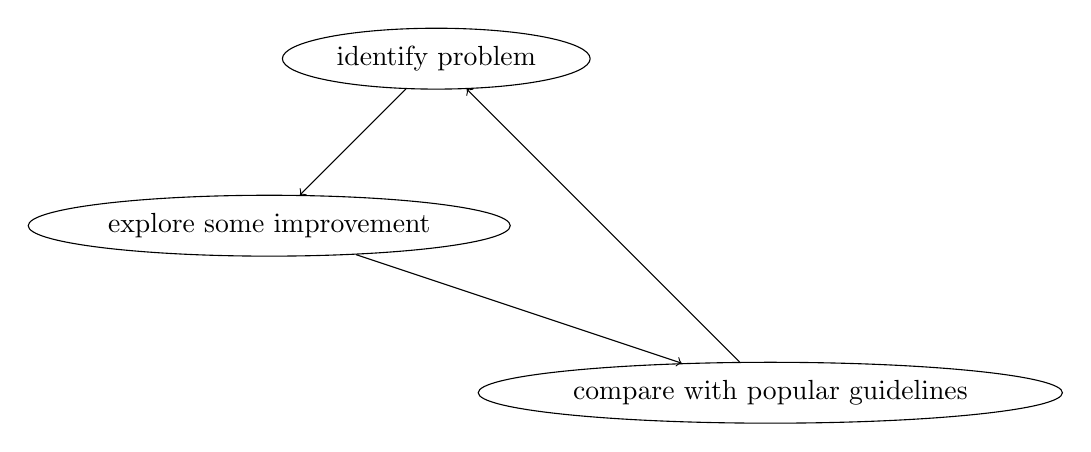
\begin{tikzpicture}[->,node distance=3cm,main node/.style={ellipse,draw}]
        \node[main node] (1) {identify problem};
        \node[main node] (2) [below left of=1] {explore some improvement};
        \node[main node] (3) [below right of=2,below right of=1] {compare with popular guidelines};

        \path[every node/.style={font=\sffamily\small}]
        (1) edge (2)
        (2) edge (3)
        (3) edge (1);
    \end{tikzpicture}
\end{frame}


\section{parser problem}

\begin{frame}[fragile]
    \frametitle{input}
    \begin{verbatim}
Location: http://www.google.com/
Content-Type: text/html; charset=UTF-8
Date: Thu, 10 Oct 2019 11:01:01 GMT
Expires: Sat, 09 Nov 2019 11:01:01 GMT
Cache-Control: public, max-age=2592000
    \end{verbatim}
\end{frame}

\begin{frame}
    \frametitle{grammar}
    \begin{columns}
        \begin{column}{.48\textwidth}
            transitions
            \begin{itemize}
                \item S $\rightarrow$ M
                \item M $\rightarrow$ L M
                \item M $\rightarrow$ e
                \item L $\rightarrow$ K : V \textbackslash n
                \item K $\rightarrow$ T
                \item V $\rightarrow$ T
                \item T $\rightarrow$ char char*
                \item char* $\rightarrow$ e
            \end{itemize}
        \end{column}
    \hfill
        \begin{column}{.48\textwidth}
            nonterminals
            \begin{itemize}
                \item S
                \item M
                \item L
                \item K
                \item V
                \item T
            \end{itemize}
        \end{column}
    \end{columns}
\end{frame}

\begin{frame}
    \frametitle{associations}
    \begin{center}
        \tikz[baseline] { \node[anchor=base,fill=red!20] {key} }
        \tikz[baseline] { \node[anchor=base,fill=green!20] {char\{:\}} }
        \tikz[baseline] { \node[anchor=base,fill=blue!20] {value} }

        \tikz[baseline] { \node[anchor=base,fill=red!20] {text} }
        \tikz[baseline] { \node[anchor=base,fill=green!20] {:} }
        \tikz[baseline] { \node[anchor=base,fill=blue!20] {hello world} }
    \end{center}
\end{frame}

\begin{frame}
    \frametitle{plan}
    \begin{enumerate}
        \item<+-> grammar generates input
        \item<+-> nonterminals represent meaning
        \item<+-> replace nonterminals with terminals
        \item<+-> compare terminals to input
        \item<+-> confirm grammar generates expected input
        \item<+-> store meaning in internal representation
    \end{enumerate}
\end{frame}


\section{parser model}

\begin{frame}
    \frametitle{parser model}
    \begin{itemize}
        \item symbols
        \item queues (symbols, input)
        \item use regular grammar to manipulate queues
    \end{itemize}
\end{frame}

\begin{frame}
    \frametitle{invariant}
    \begin{itemize}
        \item invariant: symbol stack contains unmatched symbols
        \item initialization: push start symbol on stack
        \item loop:
        \begin{itemize}
            \item pop symbol from stack
            \item find rule to match input
            \item push unknown symbols on stack
        \end{itemize}
        \item termination: if stack is empty, then grammar matched.
    \end{itemize}
\end{frame}

\begin{frame}
    \frametitle{algorithm}
    \begin{algorithm}[H]
        symbols.push(S)\;
        \While{symbols not empty and input not empty}{
            current\_symbol = symbols.pop()\;
            current\_char = input.peek()\;
            \Switch{action(current\_symbol, current\_char)}
            {
                ...\;
            }
        }
    \end{algorithm}
\end{frame}

\begin{frame}
    \frametitle{algorithm}
    \begin{algorithm}[H]
        \scriptsize
        \Case{mismatch}
        {
            symbols.push(current\_symbol)\;
            \Return\;
        }
        \Case{consumed}
        {
            input.next()\;
            symbols.push(current\_symbol)\;
        }
        \Case{finished}
        {
            \If{consume}
            {
                input.next()\;
            }
        }
        \Case{append\_symbols}
        {
            \ForEach{symbol in reverse(symbols to add)}
            {
                symbols.push(symbol)\;
            }
        }
    \end{algorithm}
\end{frame}


\section{solution}

\subsection{solution c}

\begin{frame}
    \frametitle{solution c}
    \begin{columns}
        \begin{column}{.48\textwidth}
            problems
            \begin{itemize}
                \item magic numbers
                \item details obscure logic
                \item null-terminated strings
                \item global accumulators
            \end{itemize}
        \end{column}
        \begin{column}{.48\textwidth}
            improvements
            \begin{itemize}
                \item string container
                \item stack container
                \item enum class
            \end{itemize}
        \end{column}
    \end{columns}
\end{frame}

\subsection{solution c++}

\begin{frame}
    \frametitle{solution c++ v0}
    \begin{columns}
        \begin{column}{.48\textwidth}
            problems
            \begin{itemize}
                \item big switch
                \item enum class
                \item global accumulators
            \end{itemize}
        \end{column}
        \begin{column}{.48\textwidth}
            improvements
            \begin{itemize}
                \item symbol sum type
                \item pattern matching
            \end{itemize}
        \end{column}
    \end{columns}
\end{frame}

\begin{frame}
    \frametitle{solution c++ v1}
    problems
    \begin{itemize}
        \item overloaded
        \item visit
        \item global accumulators
    \end{itemize}
\end{frame}

\begin{frame}[fragile]
    \frametitle{pattern matcher}
    \begin{minted}{c++}
struct matcher
{
    void operator()(int);
    void operator()(struct A);
    template<typename T> void operator()(std::vector<T>);
};
    \end{minted}
\end{frame}

\begin{frame}[fragile]
    \frametitle{overloaded}
    \begin{minted}{c++}
template<typename ... Ts>
struct overloaded : Ts...
{
    using Ts::operator()...;
};

template<typename ... Ts>
overloaded(Ts...) -> overloaded<Ts...>;
    \end{minted}
\end{frame}

\begin{frame}
    \frametitle{templates}
    \begin{itemize}
        \item glorified macros
        \item syntax over semantics
        \item discouraged
    \end{itemize}
\end{frame}

\begin{frame}
    \frametitle{solution c++ v1}
    improvements
    \begin{itemize}
        \item procedural paradigm
        \item internal representation
        \item simple context
    \end{itemize}
\end{frame}

\begin{frame}
    \frametitle{solution c++ v2}
    \begin{columns}
        \begin{column}{.48\textwidth}
            problems
            \begin{itemize}
                \item control coupling
            \end{itemize}
        \end{column}
        \begin{column}{.48\textwidth}
            improvements
            \begin{itemize}
                \item generic input
            \end{itemize}
        \end{column}
    \end{columns}
\end{frame}


\begin{frame}
    \frametitle{solution c++ v3}
    \begin{columns}
        \begin{column}{.48\textwidth}
            problems
            \begin{itemize}
                \item control coupling
            \end{itemize}
        \end{column}
        \begin{column}{.48\textwidth}
            improvements
            \begin{itemize}
                \item separate concerns
                \begin{itemize}
                    \item parsing
                    \item input control
                \end{itemize}
            \end{itemize}
        \end{column}
    \end{columns}
\end{frame}

\begin{frame}
    \frametitle{solution c++ v4}
    \begin{columns}
        \begin{column}{.48\textwidth}
            problems
            \begin{itemize}
                \item global accumulators
                \item semi union
            \end{itemize}
        \end{column}
        \begin{column}{.48\textwidth}
            improvements
            \begin{itemize}
                \item parse sum type
            \end{itemize}
        \end{column}
    \end{columns}
\end{frame}

\begin{frame}
    \frametitle{solution c++ v5}
    \begin{columns}
        \begin{column}{.48\textwidth}
            problems
            \begin{itemize}
                \item global accumulators
            \end{itemize}
        \end{column}
        \begin{column}{.48\textwidth}
            improvements
            \begin{itemize}
                \item closures
            \end{itemize}
        \end{column}
    \end{columns}
\end{frame}

\begin{frame}
    \frametitle{solution c++ v6}
    \begin{columns}
        \begin{column}{.48\textwidth}
            problems
            \begin{itemize}
                \item parser internal state
            \end{itemize}
        \end{column}
        \begin{column}{.48\textwidth}
            improvements
            \begin{itemize}
                \item separate data from behaviour
                \item parser trait
            \end{itemize}
        \end{column}
    \end{columns}
\end{frame}

\begin{frame}
    \frametitle{solution c++ v7}
    \begin{columns}
        \begin{column}{.48\textwidth}
            problems
            \begin{itemize}
                \item parser internal state
                \item does not preserve invariant
            \end{itemize}
        \end{column}
        \begin{column}{.48\textwidth}
            improvements
            \begin{itemize}
                \item reintroduce symbols
                \item parse symbols not input
            \end{itemize}
        \end{column}
    \end{columns}
\end{frame}

\begin{frame}
    \frametitle{solution c++ v8}
    \begin{columns}
        \begin{column}{.48\textwidth}
            problems
            \begin{itemize}
                \item manipulate frame
                \item big while
            \end{itemize}
        \end{column}
        \begin{column}{.48\textwidth}
            improvements
            \begin{itemize}
                \item symbol character
            \end{itemize}
        \end{column}
    \end{columns}
\end{frame}

\begin{frame}
    \frametitle{solution c++ v9}
    \begin{columns}
        \begin{column}{.48\textwidth}
            problems
            \begin{itemize}
                \item 350 lines
                \item big while
            \end{itemize}
        \end{column}
        \begin{column}{.48\textwidth}
            improvements
            \begin{itemize}
                \item divide
                \item makefile
                \item parser table
            \end{itemize}
        \end{column}
    \end{columns}
\end{frame}

\begin{frame}
    \frametitle{solution c++ v10}
    problems
    \begin{itemize}
        \item big while
    \end{itemize}
\end{frame}


\section{shifting perspectives}

\begin{frame}
    \frametitle{developer}
    \begin{itemize}
        \item facilities
        \begin{itemize}
            \item build
            \item debug
            \item distribute
        \end{itemize}
        \item support
        \begin{itemize}
            \item libraries
            \item community
        \end{itemize}
        \item market demands
        \item attitude "we are not c++ commitee"
    \end{itemize}
\end{frame}

\begin{frame}
    \frametitle{programmer}
    \begin{itemize}
        \item correctness
        \begin{itemize}
            \item invariant
            \item model
        \end{itemize}
        \item asymptotic complexity
    \end{itemize}
\end{frame}

\section{rust}

\begin{frame}[fragile]
    \frametitle{enum}
    \begin{minted}{rust}
enum Symbol
{
    Message,
    Line,
    Key,
    Value,
    Character(char)
}
    \end{minted}
\end{frame}

\begin{frame}[fragile]
    \frametitle{trait}
    \small
    \begin{minted}{rust}
impl std::fmt::Display for Symbol
{
    fn fmt(&self, f: &mut std::fmt::Formatter)
        -> std::fmt::Result
    {
        match self
        {
            Symbol::Message => write!(f, "Symbol::Message"),
            Symbol::Line => write!(f, "Symbol::Line"),
            Symbol::Key => write!(f, "Symbol::Key"),
            Symbol::Value => write!(f, "Symbol::Value"),
            Symbol::Character(ch)
                => write!(f, "Symbol::Character '{}'", ch),
        }
    }
}
    \end{minted}
\end{frame}

\section{state machine}

\begin{frame}
    \frametitle{fsm traits}
    \begin{itemize}
        \item fsm::store(M \& m, S s)
        \item fsm::dispatch(M \& m, E e)
        \item fsm::transit(M \& m, S \& s, E e)
    \end{itemize}
\end{frame}

\end{document}
